\chapter{Test Beam setup}\label{chap:testbeam_setup}

%%% motivate testbeam
A typical way to test the performance of sensors for High-Energy Physics applications is with test beams: the Devices Under Test (DUTs) are put through a focused flux of high energy particles and their response is read out and analyzed. %%% aka testbeam

The HGTD collaboration has run many test beam campaigns, mainly at CERN and at DESY (Deutsches Elektronen-Synchrotron). The focus of this analysis is the test beam campaign of May 2023, conducted at CERN using a beam of \qty{120}{\giga\electronvolt} pions, provided by SPS.

\begin{figure}[h!tbp]
    \centering
    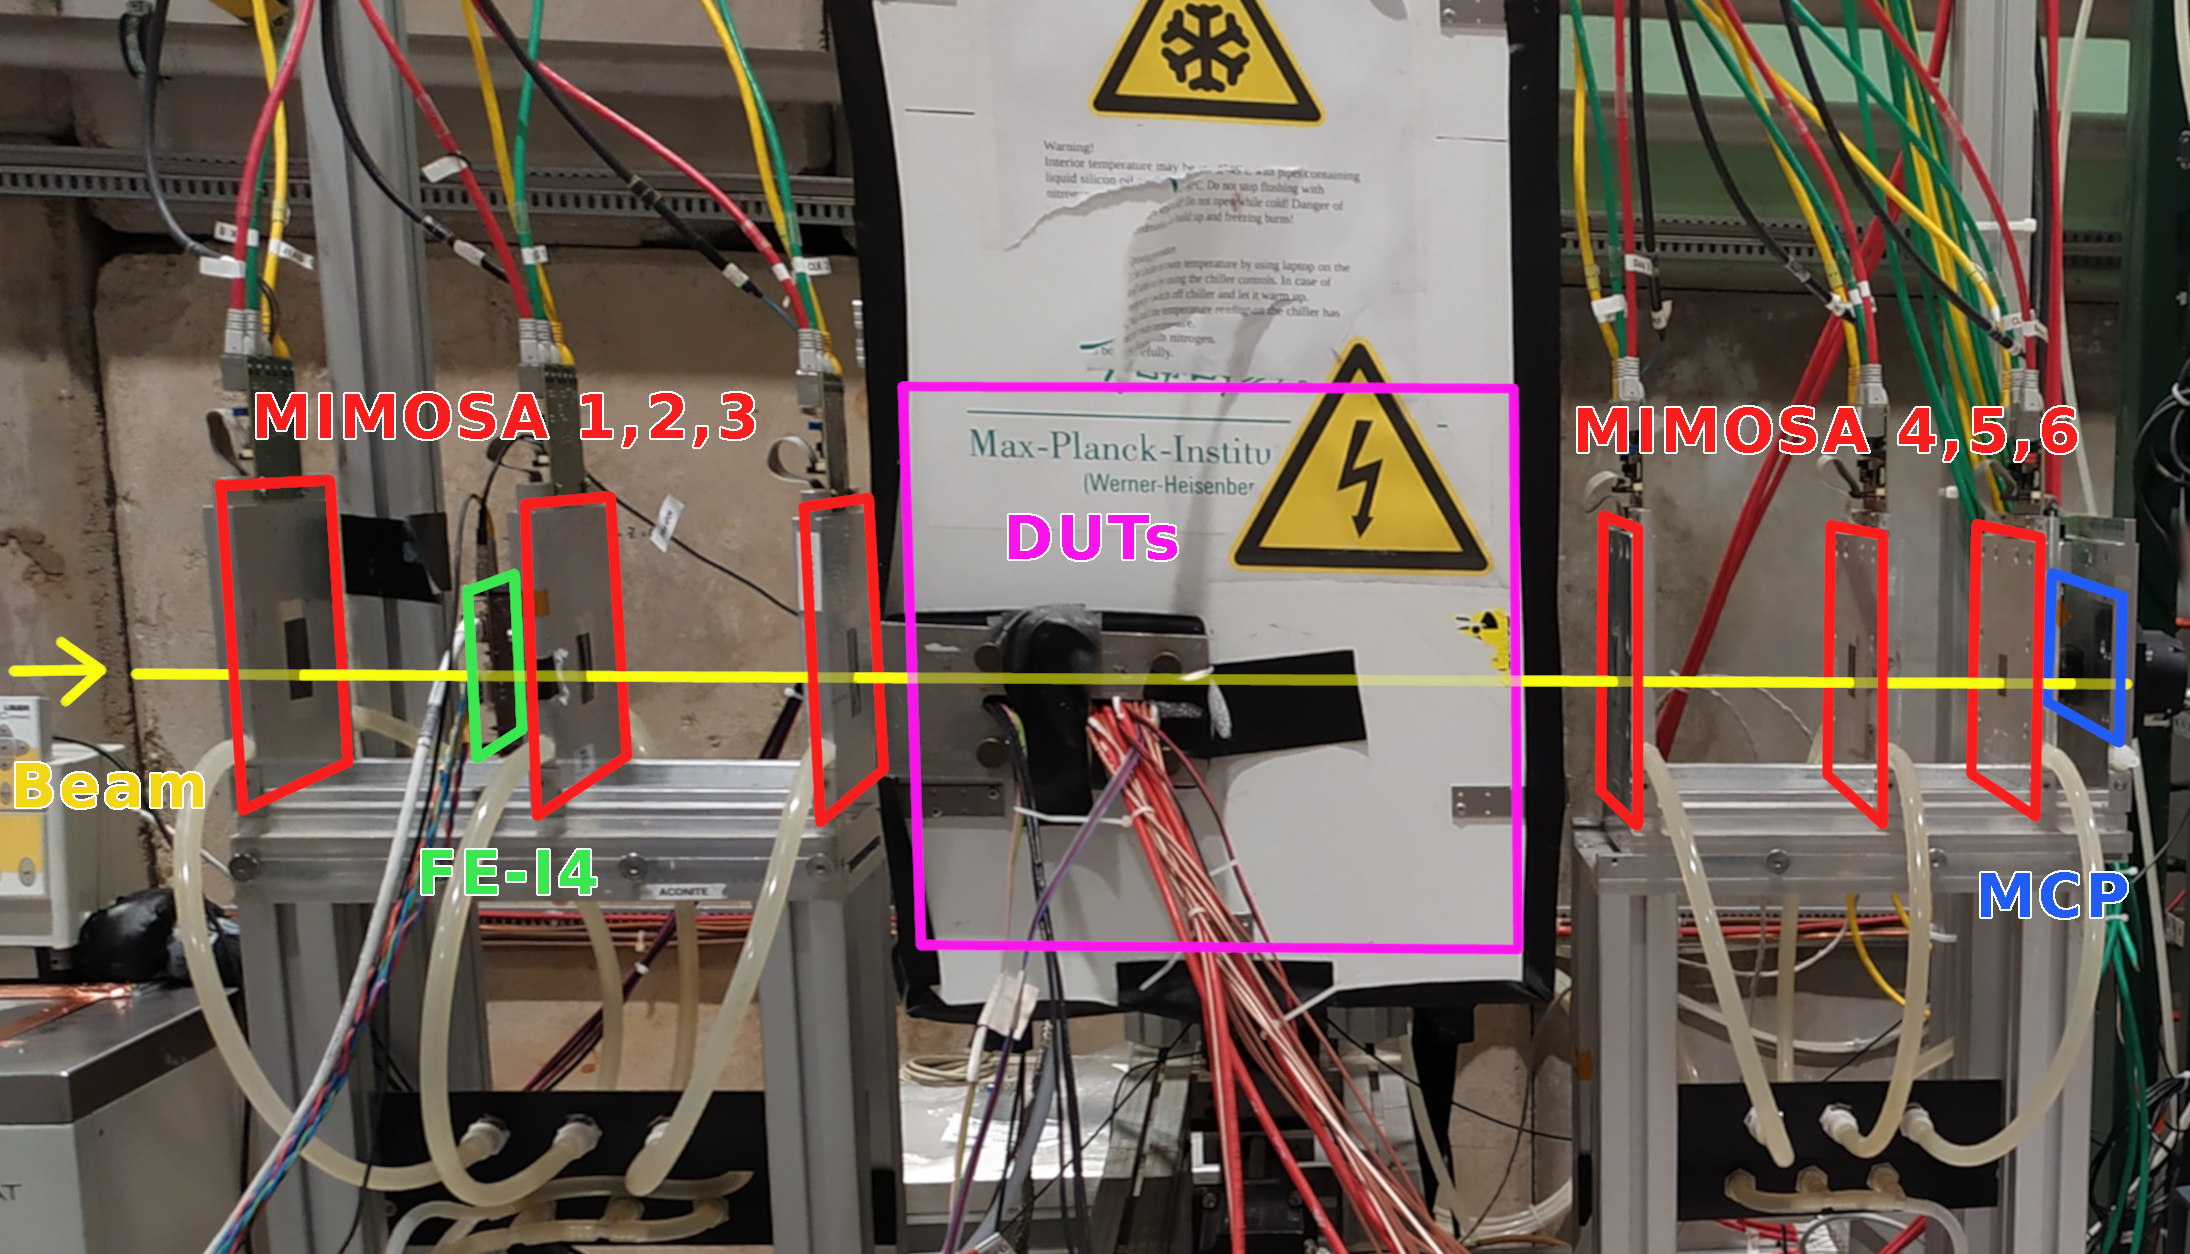
\includegraphics[width=.95\linewidth]{Images/TestBeam_setup/TestBeam_setup_redrawn.png}
    \captionsetup{width=\captionwidth}
    \caption{The main components of the test beam setup: the EUDET-type beam telescope with six MIMOSA planes, the FE-I4, the MCP and the cooling box containing the DUTs}
    \label{fig:testbeam_setup}
\end{figure}

The experimental setup of this campaign included:
\begin{itemize}
    \item FE-i4~\cite{Obermann:2014goa}: a hybrid pixel detector that provided a user-defined Region Of Interest (ROI), creating a HitOR\footnote{A binary signal generated when at least one pixel registers a hit} signal. %to avoid noisy pixels.
    \item Trigger Logic Unit (TLU): provided a trigger\footnote{A trigger is a signal that initiates data readout when a particle is detected}, combining the signals from a scintillator and the FE-i4. %% describe trigger??
    \item EUDET-type beam telescope equipped with 6 MIMOSA planes~\cite{Jansen:2016bkd}: used for precise spatial measurements of the particles in the beam, enabling track reconstruction.
    \item MicroChannel Plate detector (MCP)~\cite{LADISLASWIZA1979587}: measured the time of the moving particles, used as reference for the time resolution.
    \item Cooling box: contained the various DUTs, maintaining them at \qty{-30}{\degreeCelsius}.
    \item 2 oscilloscopes: acquired the data from the MCP and the DUTs. %%% I put later the channels
\end{itemize}

%%% maybe this should just be later

% description of components:
% • Trigger logic unit for particle passing
% • FEi4 to select a region of interest
% • Mimosa planes for tracking (X and Y position data)
% • MCP for time reference 
% • Cooling box containint the DUTs, (can be tilted with respect to the beam direction)
% • 120 GeV beam of pion

\section{TLU and FEi4}

The Trigger Logic Unit provided a trigger whenever a particle was detected. This trigger in turn instructed various components (in this case the oscilloscopes, the MIMOSA planes) to initiate data acquisition. More specifically the TLU took input from a scintillator and the FE-i4 to create a trigger.

The FE-i4 (Front-End-Iteration 4)~\cite{Obermann:2014goa} is a pixel readout chip with a planar silicon sensor bump bonded to it. It has a configurable sensitive area of up to \(\num{16.8} \times \qty{20}{\milli\meter^2}\) made up of 80 columns (\qty{250}{\micro\meter} pitch) and 336 rows (\qty{50}{\micro\meter}). 

Selecting a specific ROI allowed to exclude the areas outside the DUTs surface and to reduce sources of noise (e.g. noisy pixels of MIMOSA planes). %%% maybe the next part is just a repetition of what I say later
%It should be noted that in some occasions, due to erroneous ROI selection or due to small positional shifts caused by temperature fluctuations, the DUTs fell outside said ROI and the analysis was negatively impacted. (Example in Appendix, later)

\section{EUDET-type beam telescope}
A EUDET-type beam telescope~\cite{Jansen:2016bkd} equipped with a total of 6 Minimum Ionizing MOS Active Pixel Sensor planes~\cite{Hu-Guo:2010lrq} provided precise spatial measurements of particle trajectories. Each plane consists of 576 rows and 1152 columns of pixels, each sized \(\qty{18.4}{\micro\meter} \times \qty{18.4}{\micro\meter}\), covering an active area of around \(\num{21.2} \times \qty{10.6}{\micro\meter^2}\). Three of the planes were located before the DUTs, in the direction of the beam, and three were located after. The hits provided by the planes enabled the reconstruction of the tracks of the particles in the beam.

\section{MCP}\label{sec:MCP_description}
The microchannel plate (MCP) detector~\cite{LADISLASWIZA1979587} consists of a single block of resistive material with numerous evenly spaced small tubes (microchannels) connecting one face to the other. The main working principle is similar to that of an electron multiplier. When a voltage is applied between the two sides a potential gradient is established along the channels. Whenever a charged particle hits the inner wall of the tubes multiple secondary electrons are emitted, these electrons then are accelerated and hit the opposite wall in the channel, causing the emission of further secondary electrons. As a result, an exponentially increasing number of electrons can be extracted from the output. This detector can provide very fast response time and, for this reason, it was used as a reference for the time resolution of the other devices.


\begin{figure}
\begin{minipage}[c]{.45\linewidth}
    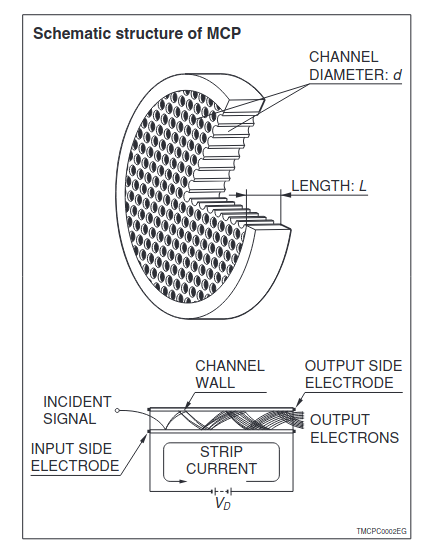
\includegraphics[width=1\linewidth]{Images/TestBeam_setup/MCP diagram HAMAMATSU.png}
\end{minipage}
\hfill
\begin{minipage}[c]{.5\linewidth}
    \caption{
    Schematics of an MCP.\\ 
    Top: structure of the detector with a cross-sectional view of the channels, highlighting the diameter \(d\) and the length \(L\) of the micro-channels. Standard MCPs are fabricated with a diameter of \(10\)s \unit{\micro\meter} and a ratio \(\alpha\) (\(\alpha = L / d\)) 40 to 60.\\
    Bottom: when a voltage (\(V_D\)) is applied, the channel walls behave as continuous electron multiplier: when a target object (electron, ion or photon) hits the inner walls, electrons are released in a parabolic trajectory, and they start a chain reaction which produces a signal amplified by \(10^4-10^7\) times. From~\cite{MCP_figure}.}
\end{minipage}
\label{fig:MCP_diagrame}
\end{figure}


\subsection{Time resolution of the MCP}
The time resolution of the MCP was first calculated by comparing the time difference of two independent sensors (CNM-W4 and CNM-W5, described in Section~\ref{sec:the_sensors}) and the MCP. In this way, it was possible to build a system of three equations of the time differences.

\begin{equation}\label{eq:time_res_system_eqs}
    \begin{cases}
        t_{1-2} = t_1 - t_2  \\
        t_{1-MCP} = t_1 - t_{MCP} \\
        t_{2-MCP} = t_2 - t_{MCP} \, .
    \end{cases}
\end{equation}

The time distributions (left sides of the equations) were fitted with a Gaussian function, each with a width \(\sigma_{ij} = \sigma_i \oplus \sigma_j\), where \(i\) and \(j\) are two of the devices in Equation~\ref{eq:time_res_system_eqs} (i.e. MCP, CNM-W4 and CNM-W5). Assuming that the devices were all independent, their time resolutions would also be independent. This gave a system of three equations with three unknowns, which could be solved analytically to find each individual time resolution: \(\sigma_1\), \(\sigma_2\), \(\sigma_{MCP}\).

This procedure was repeated for all available runs, and the results computed this way are shown in Table \ref{tab:MCP_time_resolution}.
\begin{table}[h!tbp]
    \begin{center}
        \captionsetup{width=\captionwidth}
        \caption{Time resolution values of the MCP. The uncertainty is the standard deviation of all the computed runs.}
        \label{tab:MCP_time_resolution}
        \begin{tabular}{ | c | c | c | c | }
            \hline
            Voltage [\(\si{V}\)] & 2500 & 2600 & 2800 \\ 
            \hline 
            Time resolution [\(\si{ps}\)] & 36.52 & 16.48 & 3.73 \\  
            Uncertainty [\(\si{ps}\)] & \(\pm\)0.81 & \(\pm\)0.57 & \(\pm\)1.33 \\
            \hline
        \end{tabular}
    \end{center}
\end{table}


\section{Oscilloscopes}
The signal generated by the DUT was recorded by two four-channel oscilloscopes: channel 1 (denoted as Ch1) of both oscilloscopes was connected to the MCP (whose signal was put through a splitter and sent to both oscilloscopes). Therefore, up to 6 channels were available in each batch to be attached to the DUTs.
The waveforms recorded by the oscilloscopes were then processed with the PyAna software~\cite{atlas_hgtd_pyana_2025}. 
%  \marginpar{\flushleft I explain this later in the methods}


\section{The sensors}\label{sec:the_sensors}
A variety of LGADs were tested: with different manufacturers, different designs and different fluence\footnote{Radiant exposure, here measured in neutron-equivalent over square centimeters}. They were divided into three main categories:
\begin{itemize}
    \item USTC: from the University of Science and Technology of China.
    \item IHEP: from the Institute of High Energy Physics, China.
    \item CNM: from the Centro Nacional de Microelectr\'onica, Barcelona, Spain.
\end{itemize}

The first two designs have both been manufactured by the IME (Institute of Microelectronics) of the Chinese Academy of Sciences. The two unirradiated CNM sensors (labeled CNM-W4 and CNM-W5) were used to measure the time resolution of another device, the MCP (Section~\ref{sec:MCP_description}), which was used as a time reference for the time measurements of all the other LGADs. 

Two other devices from CNM were irradiated at \qty{1.5e15}{\neutroneq} and \qty{2.5e15}{\neutroneq}. Two versions (v2 and v3) of the IME-IHEP sensors were available, both had a carbon implantation, which has the purpose of increasing the radiation hardness of the LGAD. The sensors were either a single pad or an array (2\(\times\)2 or 1\(\times\)3) of pads, and they were irradiated at fluences ranging from \(0\) to \qty{2.5e15}{\neutroneq}. Two USTC devices, also with carbon enrichment (version 2.1), were tested at zero and low fluence. 

Notably, the data from the irradiated USTC sensor was not available. Moreover, one pad of IMEv3-W12-2x2-1.5E15 was removed from the analysis due a possible wrong labeling (see in Appendix~\ref{sec:mislabeled_sensor}).

The sensors were then installed onto readout boards. In the case of multi-pads sensors, some number of pads were each connected to one channel of the board, so that they could be measured individually.

Table \ref{tab:devices_tested} provides the list of the devices that were characterized.

%%% for more detailed descriptions see Table in \nameref{chap:appendix}.
%%% TODO: maybe more complete table in appendix? with devices id

\begin{table}[h!tbp]  
    \centering
    \captionsetup{width=\captionwidth}
    \caption{List of the tested devices.}
    \label{tab:devices_tested}

    % \makebox[1\textwidth][c]{
    \begin{tabular}{|l|l|l|l|l|l|}
    \hline %%% I NEED TO TRY TO USE TABULAR INSTEAD OF SHORTSTACK
        \textbf{Device name} & \textbf{Vendor} & \begin{tabular}{@{}l@{}}\textbf{Pads,} \\ \textbf{used channels}\end{tabular} & \begin{tabular}{@{}l@{}}\textbf{Fluence} \\ \([n_{eq}/\si{cm^2}]\) \end{tabular} & \begin{tabular}{@{}l@{}} \textbf{Radiation} \\ \textbf{type} \footnotemark \end{tabular}& \textbf{Notes} \\
        \hline
        CNM-W4  & CNM & single & 0 & - & reference \\ 
        CNM-W5  & CNM & single & 0 & - & reference \\ 
        CNM-W5-1.5E15  & CNM & single & \(\num{1.50E+15}\) & neutron & - \\ 
        CNM-W3-2.5E15  & CNM & single & \(\num{2.50E+15}\) & neutron & - \\ 
        USTC2.1-W17 & USTC & 2\(\times\)2, 2 channels  & 0 & - & - \\ 
        USTC2.1-W17-2E14 & USTC & 2\(\times\)2, 1 channel & 0 & - & not available\\ 
        IMEv3-W12-2x2  & IHEP & 2\(\times\)2, 2 channels  & 0 & - & \\ 
        IMEv3-W12-1x3  & IHEP & 1\(\times\)3, 2 channels  & 0 & -  &\\ 
        IMEv3-W12-2x2-1.5E15 & IHEP & 2\(\times\)2, 3 channels  & \(\num{1.50E+15}\) & neutron & only two channels \\ 
        IMEv2-W7-1E14  & IHEP & single & \(\num{1.00E+14}\) & proton & -\\ 
        IMEv2-W7-6.5E14  & IHEP & single & \(\num{6.50E+14}\) & proton  & - \\ 
        IMEv3-W16-8E14  & IHEP & single & \(\num{8.00E+14}\) & proton & - \\
        IMEv3-W16-1x3-1.5E15  & IHEP & 1\(\times\)3, 1 channel  & \(\num{1.50E+15}\) & neutron & no usable batches \\ 
        IMEv3-W16-2.5E15  & IHEP & single & \(\num{2.50E+15}\) & neutron  & - \\ 
        \hline
    \end{tabular}
\end{table}

\footnotetext{\label{footnote:radiation_type} As protons and neutrons interact differently with the atoms of the silicon lattice, they can introduce distinct defect structures. In addition, the enrichment of various impurities may lead to further differences in the type of damage \cite{Ruzin:1999ck}.}

%%% NOT UPDATED ANYMORE, LOOK AT THE EXCEL FILE, I MIGHT DELETE THIS LATER
%%% I have to reorganize these and associate them with the more accurate descriptions
% device name:        vendor:        sensor ID:            fluence:    irradiation type:    type:        board name:    channels:
% CNM-W4              CNM          CNM-R15973-W4-D168      unirradiated      -             single pad     JSI-B12      1
% CNM-W5              CNM          CNM-R15973-W5-D138      unirradiated      -             single pad     JSI-B14      1
% CNM-W3-2.5E15       CNM          CNM-R15973-W3-D29       $\num{2.5e15}     neutron       single pad     JSI B5       1
% CNM-W5-1.5E15       CNM          CNM-R15973-W5-D29       $\num{1.5e15}     neutron       single pad     JSI PP1      1
% USTC2.1             USTC         USTC2.1-W17-P6-A          0                -             2\(\times\)2           CERN-3       1,2
% USTC2.1 IRRADIATED (MISSING)
% IMEv3-W12-C2         IHEP        IMEv3-W12-C2-2-2          0               -              2\(\times\)2          CERN-1       channels 1,2
% IMEv3-W12-C3         IHEP        IMEv3-W12-C3-1-4 (and 5)  0               -              1x3          CERN-1       channles 3,4  (small GR), bonded
% CERN2-CH0-IMEv3-W12  IHEP        IMEv3-W12-B2-2-9-1       1.5e15           neutron        2\(\times\)2 sensor    CERN-2       channels 1,2,3
% CERN2-CH1-IMEv3-W12  IHEP 
% CERN2-CH2-IMEv3-W12  IHEP 
% CERN2-CH4-IMEv3-W16  IHEP        IMEv3-W16-Q4-D4-1-4      1.5e15           neutron        1x3          CERN-2       channel:  2(?)
% JSI-B6-IMEv2-W7-1E14    IHEP       W7-II-C2-1-7 IMEv2-W7Q2    1e14          proton        single       JSI-B6
% JSI-PP4-IMEv2-W7-6.5E14 IHEP       W7-II-C2-1-7 IMEv2-W7Q2    6.5e14        proton        single       JSI-PP4
% JSI-B7-IMEv3-W16-8E14   IHEP       IHEP-IMEv3-W16_Q4_D3_1-4   8e14          (unsure)        single       JSI-B7
% JSI-B13-IMEv3-W16-2.5E15 IHEP      IHEP-IMEv3-W16_Q4_E3_1-4   2.5e15       (unsure)      single        JSI-B13
                 